\documentclass[11pt]{beamer}
\usepackage[UTF8, noindent]{ctex}
\usepackage{indentfirst}
\setlength{\parindent}{2em}



% some package
% graph
\usepackage{graphicx}
\RequirePackage{subfigure}
\RequirePackage{float}
% math
\RequirePackage{amsmath}
\RequirePackage{amssymb,amsfonts,mathrsfs}

\RequirePackage{bm}         % \mathbf{}
\RequirePackage{color}      % the color of the font
\usepackage{mathrsfs}
\RequirePackage{enumerate}

% theme
\usetheme{Antibes}
\usecolortheme{lily}
\usefonttheme{serif}
%\usefonttheme{professionalfonts}

% the caption of thf figure
\renewcommand{\figurename}{图}
\setbeamertemplate{caption}[numbered]

% font
%\setCJKmainfont{SimSun}
%\setmainfont{Consolas} 

\title{复杂网络}
\institute{计算机学院}
\author{高一鸣 \ 王方正 \ 邵逸岚 \ 庞冰瑶 \ 赵帅 \ 张永辉}
\date{2018.04.27}

\begin{document}
	

	\begin{frame}
		\titlepage
	\end{frame}

	\section*{复杂网络基础}

\begin{frame}
	\centerline{\textbf{\Large{复杂网络基础}}} 
	~\\
	\centerline{\large{赵帅}}
\end{frame}

\subsection*{什么是复杂网络}

	\begin{frame}
		\frametitle{什么是复杂网络?}
	
		\begin{itemize}
		\item 在网络理论的研究中,复杂网络是由数量巨大的节点和节点之间错综复杂的关系共同构成的网络结构。用数学的语言来说,就是一个有着足够复杂的拓扑结构特征的图。 \\ ~\\
		\item 具有自组织、自相似、吸引子、小世界、无标度中部分或全部性质的网络称为复杂网络。
		\end{itemize}
	
	\end{frame}



	\begin{frame}
	
		\begin{figure}[htbp]
			\centering
			\begin{minipage}[t]{0.45\textwidth}
				\centering
				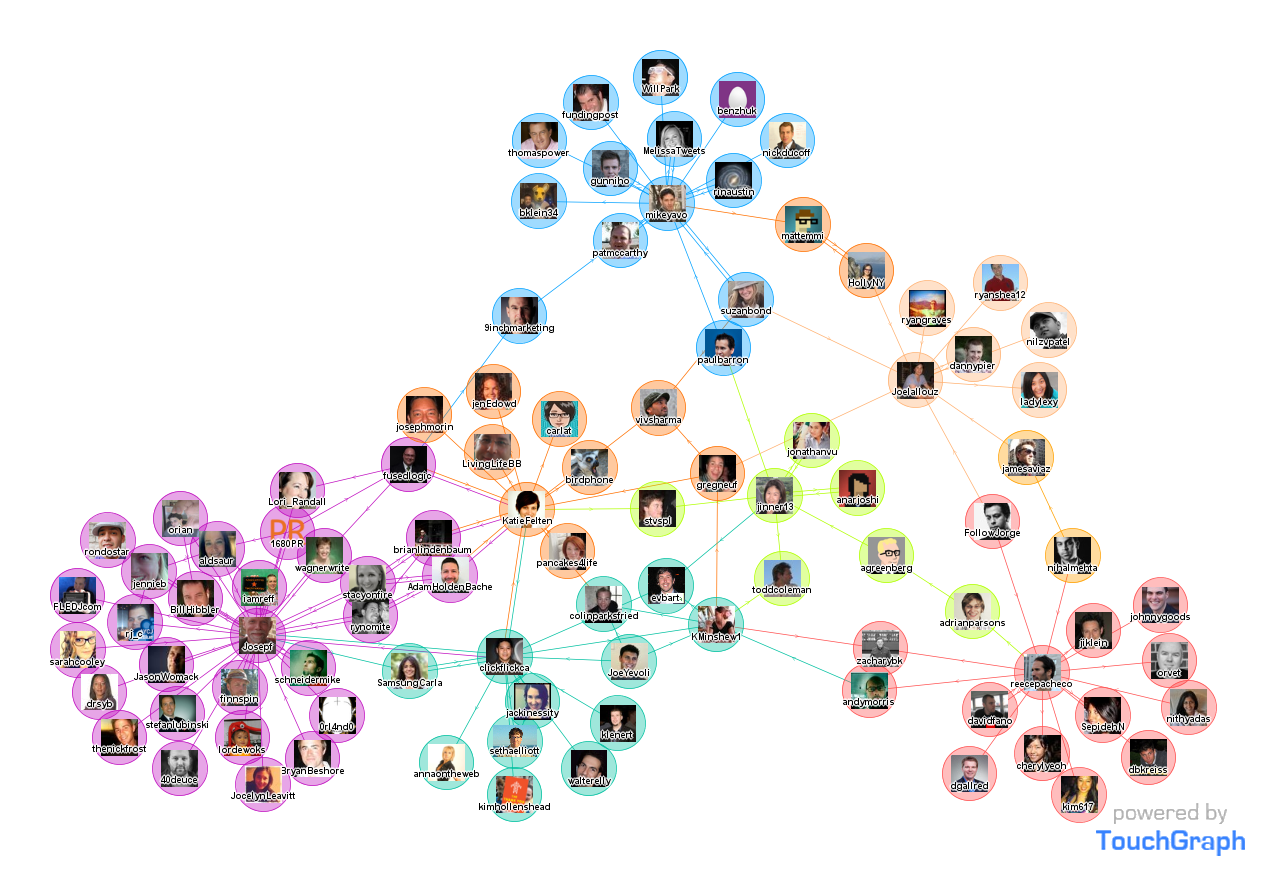
\includegraphics[height=3.5cm]{pic/01-social.png}
				\caption{社交网络}
			\end{minipage}
			\begin{minipage}[t]{0.45\textwidth}
				\centering
				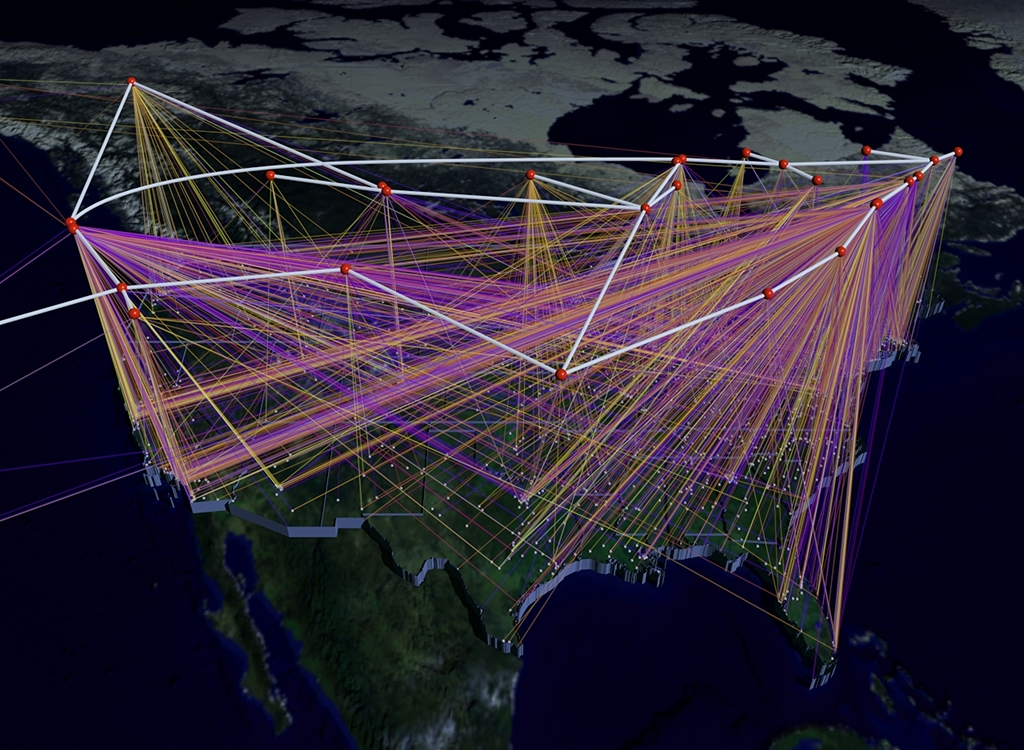
\includegraphics[height=3.5cm]{pic/01-internet.jpg}
				\caption{Internet一部分的可视化}
			\end{minipage}
		\end{figure}
	
	\end{frame}


\subsection*{网络的图表示}

	\begin{frame}
		\frametitle{网络的图表示}
			
		\begin{figure}[htbp]
			\centering
			%\flushleft
			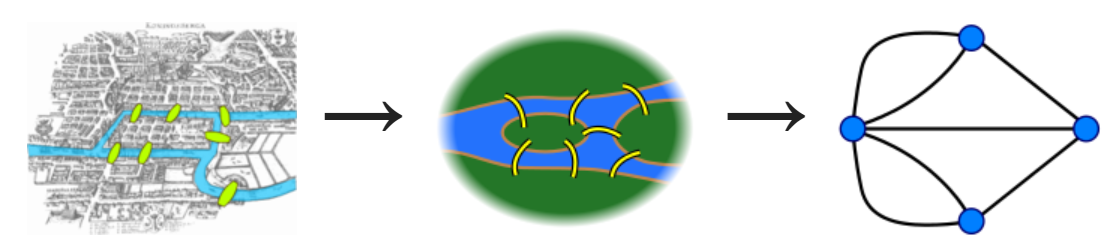
\includegraphics[width=0.6\textwidth, bb = 0 0 1116 249]{pic/01-sevenb.png}
			\caption{七桥问题-Euler图}
		\end{figure}

		图论之父-Euler. \\
		
		~\\
		一个具体网络可以抽象为一个由点集$V$和边集$E$组成的图$G=(V,E)$。节点数记为$N=|V|$,边数记为$M=|E|$。 一条边对应一对点。\\
		无向网络、有向网络、加权网络、无权网络、重边、自环。
	
	\end{frame}


\subsection*{三个指标}

\begin{frame}

	
	\begin{itemize}
		\item \textbf{平均路径长度}  \\
				网络中两个节点$i$和$j$之间的距离$d_{ij}$定义为连接这两个节点的最短路径上的边数。
				网络的直径$ D = \max\limits_{i,j}d_{ij}$ 。\\
				网络的平均长度 $L = \frac{1}{2} \frac{1}{N(N+1)}\sum\limits_{i \ge j}d_{ij}$,也叫特征长度路径。\\
		\item \textbf{聚类系数} \\
				$k_i$个节点之间最多可能有$k_i (k_i - 1)/2$条边,实际存在的边数为$E_i$ 。$ \text{聚类系数} C_i = 2E_i / k_i (k_i - 1)$ 。\\
				由其几何特点等价为 $C_i = \frac{\text{与点}i\text{相连的三角形的数量} }{\text{与点}i\text{相连的三元组的数量}}$。\\
				整个网络的聚类系数$C$就是所有节点$i$的聚类系数$C_i$的平均值。
	
	\end{itemize}

	\begin{figure}[htbp]
		\centering
		%\flushleft
		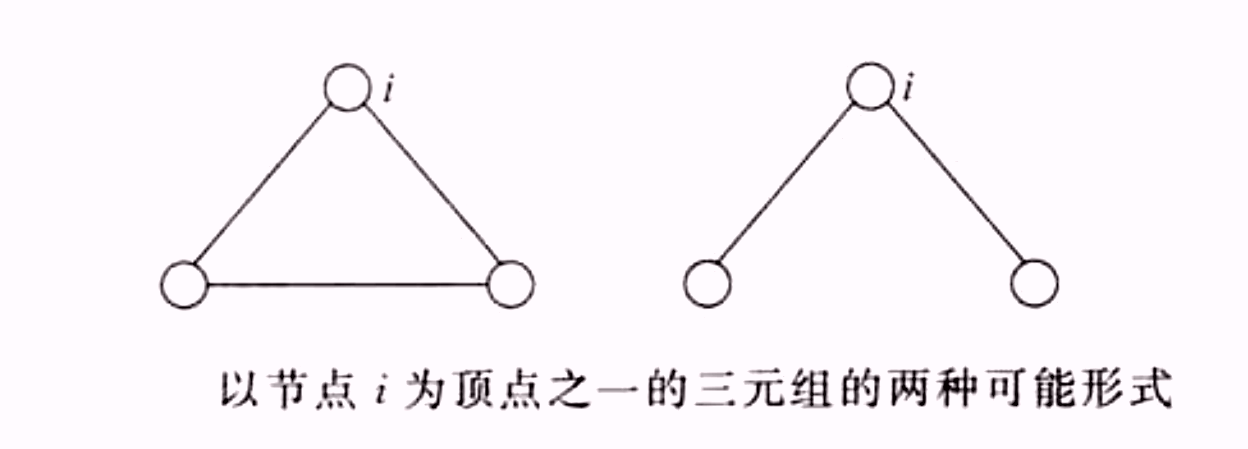
\includegraphics[width=0.6\textwidth, bb = 0 0 1248 449]{pic/01-three.png}
	\end{figure}

	

\end{frame}


\begin{frame}
	\frametitle{三个指标}
	\begin{itemize}
		\item \textbf{度与度分布}\\
				节点$i$的度定义为与该节点连接的其他节点的数目。出度(out-degree)、入度(in-degree)。\\
				度越大从某种意义上意味着该节点越重要。 \\
				所有节点$i$的度$k_i$的期望称为网络的(节点)平均度,记为$<k>$。网络中节点的度分布可用分布函数$P(k)$来描述。\\
				~\\
				\begin{itemize}
					\item \textbf{无标度条件} \\
					对概率分布函数$f(x)$,对任意常数$a$,存在常数$b$使$f(x)$满足“无标度条件”:$f(ax)=bf(x)$,那么一定有:$f(x)=f(1)x^{-\gamma}, \gamma = -f(1)/f^{\prime}(1)$。\\
					~\\
					幂律分布函数$P(k)\propto x^{-\gamma}$是唯一满足“无标度条件”的概率分布函数。
				\end{itemize}
			
	\end{itemize}
\end{frame}

\begin{frame}
	\frametitle{三个指标}
	\begin{figure}[htbp]
		\centering
		%\flushleft
		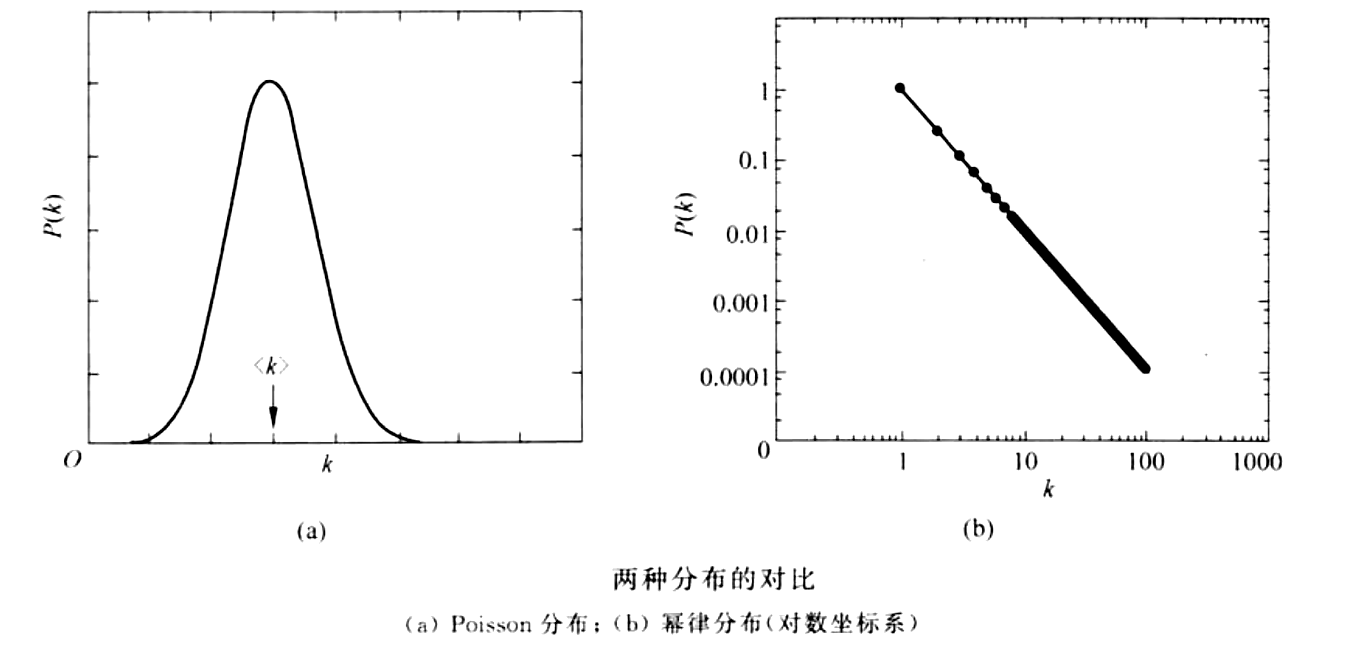
\includegraphics[width=0.95\textwidth, bb = 0 0 1365 652]{pic/01-pandp.png}
	\end{figure}
	\begin{itemize}
		\item 均匀网络:公路网等
		\item 非均匀网络:航空网、Internet等
	\end{itemize}
	
\end{frame}

\subsection*{规则网络}

	\begin{frame}
	\frametitle{规则网络}
	
		\begin{itemize}
		\item \textbf{全局耦合(coupled)网络}:任意两点均有边相连。平均路径长度$L_{gc}=1$(最小),聚类系数$C_{gc}=1$(最大)。 \\ ~\\
		\item \textbf{最近邻耦合网络}:每个节点只和周围的邻居节点相连。\\ 
				具有周期边界条件的最近邻耦合网络,$N$个点围成一个环,每个节点与左右$K/2$个点相连,$K$是偶数。对较大的$K$值,聚类系数$C_{nc}=\frac{3(K-2)}{4(K-1)}\approx\frac{3}{4}$,平均路径长度$L_{nc}\approx \frac{N}{2K} \rightarrow \infty ((N \rightarrow \infty)$。 \\ ~\\
		\item \textbf{星形耦合网络}:有一个中心点,其余$N-1$个点只与中心点相连。\\ 
				聚类系数$C_{star}=\frac{N-1}{N} \rightarrow (N \rightarrow \infty)$,平均路径长度$L_{star}=2- \frac{2(N-1)}{N(N-1)} \rightarrow 2 (N \rightarrow \infty)$。
		\end{itemize}

	\end{frame}

	\begin{frame}
		\begin{figure}[htbp]
			\centering
			%\flushleft
			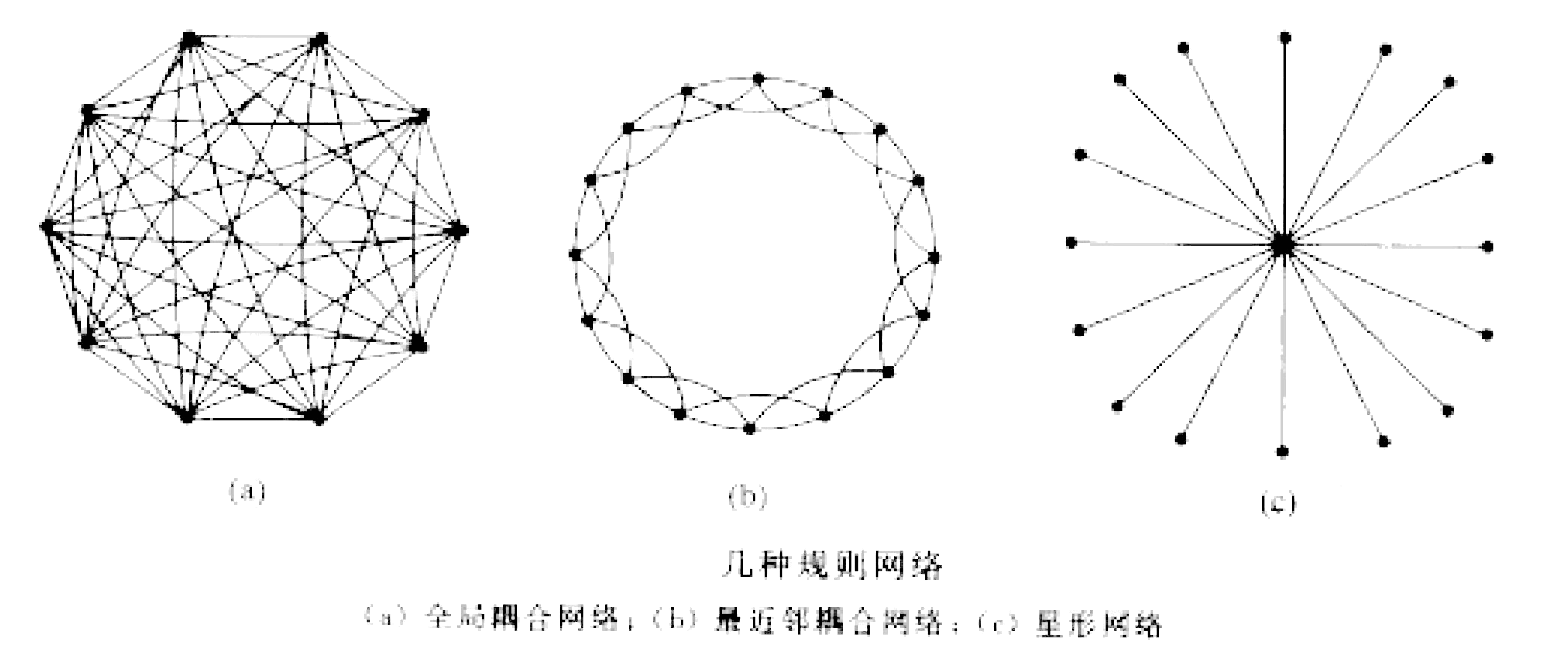
\includegraphics[width=0.95\textwidth, bb = 0 0 1548 649]{pic/01-rgraph.png}
		\end{figure}
	\end{frame}
	
\subsection*{随机网络}

	\begin{frame}
		\frametitle{随机网络}
		\begin{itemize}
			\item \textbf{ER随机网络}(Erdős–Rényi model,1959) \\ 
					$N$个点,以概率$p$在两个点之间连线而成的图。\\ ~\\
					平均度$<k> = p(N-1) \approx pN$,二项分布$\rightarrow $泊松分布($N\rightarrow \infty$)。
					平均路径长度为网络规模的对数增长函数,$L_{ER} \propto \ln N / \ln <k>$(小世界特性)。\\
					聚类系数$C=p=<k>/N \ll 1$。 \\
					与实际复杂网络模型相比存在明显缺陷。
		\end{itemize}
		
		\begin{figure}[htbp]
			\centering
			%\flushleft
			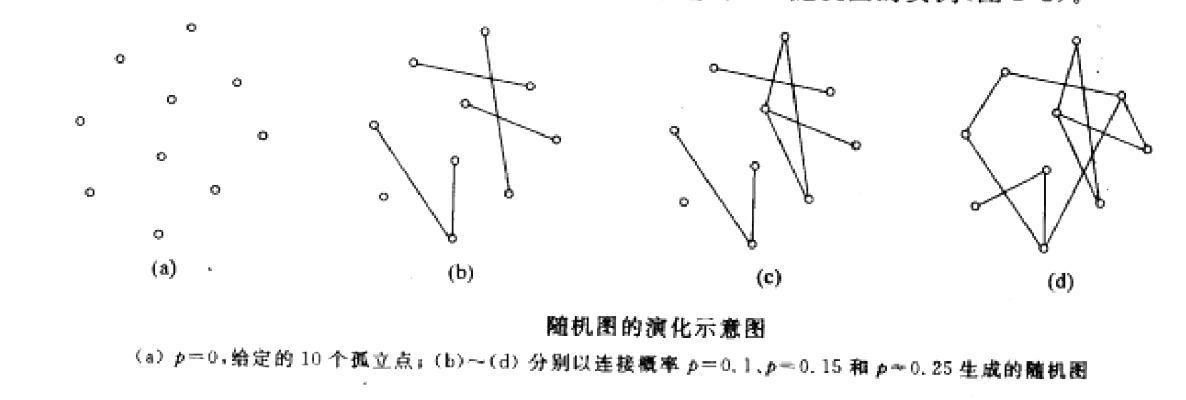
\includegraphics[width=0.7\textwidth, bb = 0 0 1186 400]{pic/01-ERgraph.png}
		\end{figure}
	\end{frame}

\subsection*{小世界网络}

	\begin{frame}
		\frametitle{小世界网络}
		\begin{itemize}
			\item \textbf{小世界网络} \\ 
			具有较短平均路径长度的同时,又具有较高的聚类系数的一类网络。
		\end{itemize}

		\begin{center}
		\fbox{
			\centering
			\parbox[tc][72pt][t]{300pt}{
				\textbf{WS小世界模型}(Watts \& Strogtz,1998) 
			\begin{enumerate}[(1)]
				\item 从规则图开始:上文所提到的最近邻耦合网络。环形,每个节点与左右相邻的$K/2$个节点相连。
				\item 随机化重连:以概率$p$随机的重新连接网络中的每条边,即边的一个端点保持不变,另一个节点在网络中随机选取。
			\end{enumerate}
		}} 
		\end{center}
		~\\
		$p=0$时,没有不同。$p$较小时,新的网络与原始网络局部属性差别不大,从而网络的聚类系数变化也不大,平均路径长度却下降很快。上文提到的小世界网络性质。
		
	\end{frame}

	\begin{frame}
	\frametitle{小世界网络}
	WS小世界模型构造算法中的随机化过程有可能破坏网络的连通性。\\
	\begin{center}
	\fbox{
		\centering
		\parbox[tc][72pt][t]{300pt}{
			\textbf{NW小世界模型}(Newman \& Watts,2000) 
			\begin{enumerate}[(1)]
				\item 从规则图开始:上文所提到的最近邻耦合网络。环形,每个节点与左右相邻的$K/2$个节点相连。
				\item 随机化加边:以概率$p$在在随机选取的一对节点之间加上一条边。任意两各节点之间至多有一条边,无自环。
			\end{enumerate}
	}}
	\end{center}
	~\\
	小世界网络反映了朋友关系网络的一些特性,大部分人的朋友都是其邻居或单位同事,但也有一些人住得很远。
	
	\end{frame}

	\begin{frame}
		\frametitle{小世界网络}
	
		\begin{figure}[htbp]
		\centering
		%\flushleft
		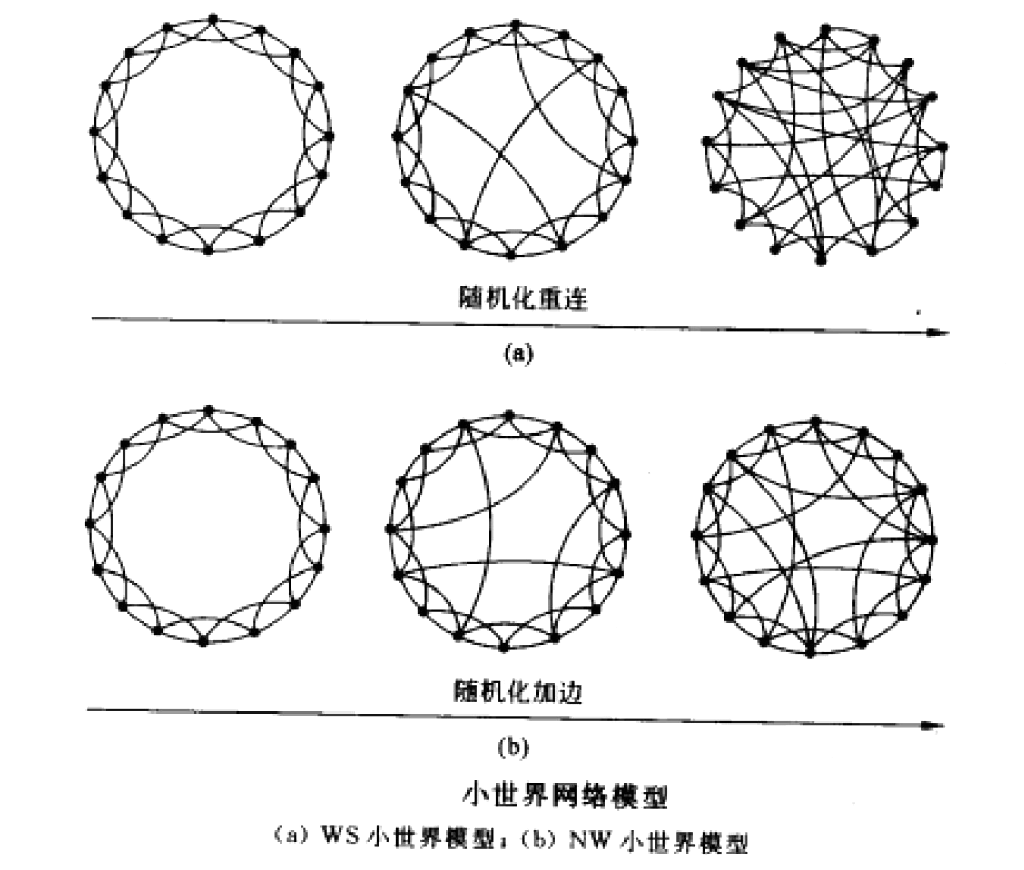
\includegraphics[width=0.75\textwidth, bb = 0 0 1024 870]{pic/01-smallw.png}
		\end{figure}
	
	\end{frame}


	\begin{frame}
		\frametitle{统计性质}
	
		\begin{itemize}
			\item 聚类系数 \\
				WS小世界网络:$C(p) = \frac{3(K-2)}{4(K-1)}(1-p)^3$ \\
				NW小世界网络:$C(p) = \frac{3(K-2)}{4(K-1) + 4Kp(p+2)}$ 
			\item 平均路径长度 \\
				没有精确的显示表达式,但有一些近似表达式。大体上,$p、K$确定的情况下,$L(p) \propto \ln N$。
			\item 度分布 \\
				大体上,二项分布,极限情况下逼近泊松分布,是所有节点的度都大致相等的均匀网络。
		\end{itemize}
		~\\
		有一些利用小波分析进行小世界网络分析的研究。
	\end{frame}

	\begin{frame}
		\frametitle{小世界网络}
		\begin{itemize}
			\item 六度分离理论 \\
			世界上任何互不相识的两人,只需要很少的中间人就能够建立起联系。\\ 
			\item Kevin Bacon游戏 \\ 
			\item Erdős 数 
		\end{itemize}
	
		\begin{figure}[htbp]
			\centering
			%\flushleft
			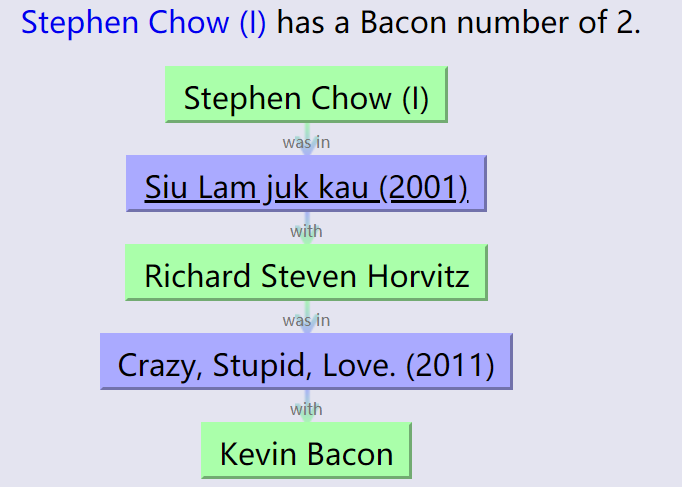
\includegraphics[width=0.5\textwidth, bb = 0 0 682 487]{pic/01-kevin.png}
		\end{figure}

	\end{frame}

\subsection*{无标度网络}

	\begin{frame}
		\frametitle{无标度网络}
		ER随机图和WS小世界模型的度分布可近似用Poisson分布表示(均匀网络或指数网络)。\\ ~\\
		许多复杂网络(Internet、新陈代谢网络)等的度分布具有幂律形式。这类网络节点的连接度没有明显的特征长度,故称为无标度网络。\\
		~\\
		为了解释幂律分布的产生机理,提出了BA模型。\\
		两个重要特性:
		\begin{itemize}
			\item 增长 \\
			网络规模不断扩大。\\ 
			\item 优先连接 \\ 
			新的节点趋向于与那些具有较高连接度的节点相连接,“马太效应”。
		\end{itemize}


	\end{frame}

	\begin{frame}
		\frametitle{BA无标度网络}	
		\begin{center}	
			\fbox{
				\centering
				\parbox[tc][130pt][t]{270pt}{
					\textbf{BA无标度模型构造算法}(Barabási \& Albert,2000) 
					\begin{enumerate}[(1)]
						\item 增长:从一个具有$m_0$个节点的网络开始,每次引入一个新的节点连接到$m$个已存在的节点上,$m\le m_0$。
						\item 优先连接:一个新节点与一个已经存在的节点$i$相连接的概率$\prod_i$与节点$i$的度$k_i$、节点$j$的度$k_j$之间满足如下关系:
						$$\prod_i = \frac{k_i}{\sum\limits_{j}k_j}$$
					\end{enumerate}
				}
			}
		\end{center}
		\begin{figure}[htbp]
			\centering
			%\flushleft
			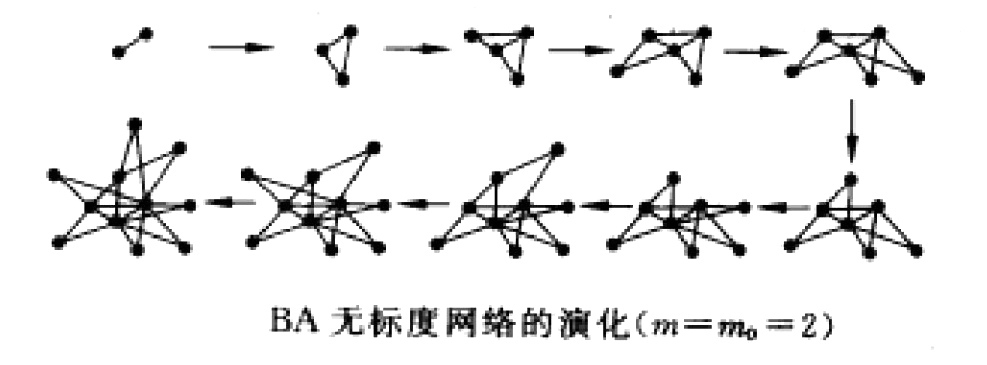
\includegraphics[width=0.6\textwidth, bb = 0 0 987 365]{pic/01-BA.png}
		\end{figure}
		
	\end{frame}

	\begin{frame}
		\frametitle{BA无标度网络}
		
		\begin{itemize} \itemsep=2ex
			\item 平均路径长度: $L \propto \frac{\log N}{\log \log N}$。具有小世界特性。 
			\item 聚类系数:没有明显的聚类特征。
			\item 度分布 :大体满足幂律分布。
		\end{itemize}
		~\\
		无标度网络的鲁棒性与脆弱性。\\ ~\\ 
		BA无标度网络中,越老的节点具有越高的度。实际网络中并非如此,有些节点由于自身的特殊性质,更容易被新新加入的节点所连接。如个人的交友能力和科研论文的质量等等。\\
	\end{frame}

	\begin{frame}
		\frametitle{适应度模型}	
		\begin{center}	
		\fbox{
			\centering
			\parbox[tc][130pt][t]{300pt}{
				\textbf{适应度模型构造算法}(Bianconi \& Barabási,2001) 
				\begin{enumerate}[(1)]
					\item 增长:从一个具有$m_0$个节点的网络开始,每次引入一个新的节点连接到$m$个已存在的节点上,$m\le m_0$。每个节点的适应度按概率分布$\rho(\eta)$选取。
					\item 优先连接:一个新节点与一个已经存在的节点$i$相连接的概率$\prod_i$与节点$i$的度$k_i$、节点$j$的度$k_j$和适应度$\eta_i$之间满足如下关系:
					$$\prod_i = \frac{\eta_i k_i}{\sum\limits_{j}\eta_i k_j}$$
				\end{enumerate}
		}}
		\end{center}
		
		适应度模型中,假如年轻的节点具有较高的适应度,在后续演化过程中会获得更多的边。\\
		适应度分布的性质不同,适应度模型会有不同的行为表现。
	\end{frame}

\subsection*{复杂网络的自相似性}

	\begin{frame}
		\frametitle{复杂网络的自相似性}
			
		局部在某种意义上与整体相似,就是自相似性。是分形的基本特征。	
			
		\begin{figure}[htbp]
			\centering
			%\flushleft
			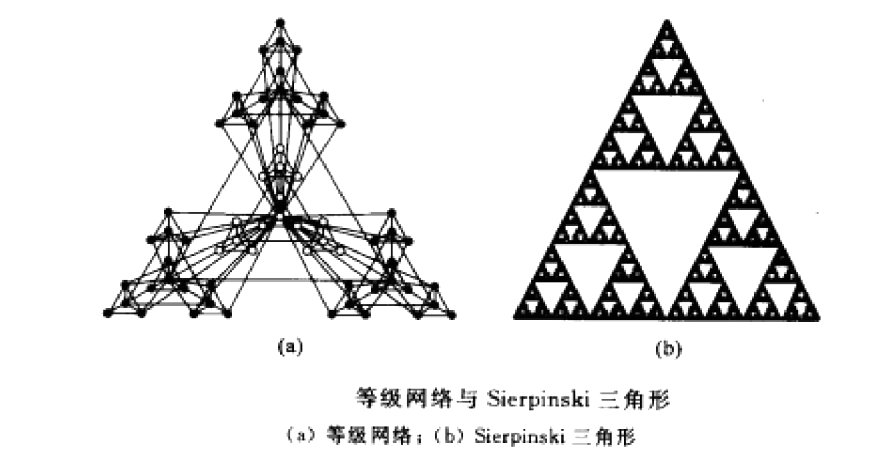
\includegraphics[width=0.6\textwidth, bb = 0 0 884 457]{pic/01-self.png}
		\end{figure}
		\textbf{盒计数法} :用边长$l_B$的盒子来完全覆盖一个几何图形,需要的最少盒子数为$N_B(l_B)$。图形的维数近似计算公式为:
		$d_B \approx - \frac{\ln N_B(l_B)}{ln(l_N)} (l_B \rightarrow 0)$。分割方式难以寻找。
		
	\end{frame}



\subsection*{自组织与吸引子}

	\begin{frame}
		\frametitle{自组织与吸引子}
		
		\begin{itemize} \itemsep=2ex
			\item \textbf{自组织} \\
					是一系统内部组织化的过程,通常是一开放系统,在没有外部来源引导或管理之下会自行增加其复杂性。\\
					自组织是从最初的无序系统中各部分之间的局部相互作用,产生某种全局有序或协调的形式的一种过程。这种过程是自发产生的,它不由任何中介或系统内部或外部的子系统所主导或控制。
			\item \textbf{吸引子}
					一个系统有朝某个稳态发展的趋势,这个稳态就叫做吸引子。吸引子分为平庸吸引子和奇异吸引子。\\
					如钟摆系统有一个平庸吸引子,其使钟摆系统向停止晃动的稳态发展。\\
					学术上并没有完善的定义,仅处于概念阶段。
		\end{itemize}

	\end{frame}


















	

	
	\section*{贝叶斯网络}

\begin{frame}
\centerline{\textbf{\Large{贝叶斯网络}}} 
~\\
\centerline{\large{邵逸岚}}
\end{frame}

\subsection*{贝叶斯定理}
\begin{frame}
	\textbf{贝叶斯公式:}
	~\\
	\centerline{{\large $P(A|B)=\frac{P(B|A)P(A)}{P(B)}$}}
	~\\
	~\\
	~\\
	后验概率=(相似度*先验概率)/标准化常量 
\end{frame}

\subsection*{定义}
\begin{frame}
	贝叶斯网络(Bayesian Network)是一种经典的概率图模型,它借助有向无环图(Directed Acyclic Graph, DAG)来刻画属性之间的依赖关系,并使用条件概率表(Conditional Probability Table, CPT)来描述属性的\textbf{联合}概率分布。
\end{frame}

\subsection*{结构}
\begin{frame}
	\begin{figure}
		\centering
		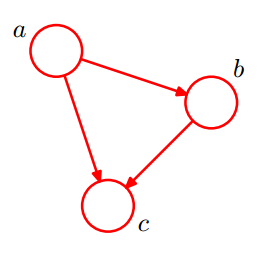
\includegraphics[scale=0.5]{pic/bn.png}
		\caption{贝叶斯网络结构图}
		\label{0-002}
	\end{figure}
\end{frame}

\begin{frame}
	贝叶斯网络B由结构G和参数$\Theta$构成,即$B=\langle G, \Theta\rangle$。给定父结点集,假设每个属性与它的非后裔属性独立,于是将属性$x_1, x_2, ..., x_d$的联合概率分布定义为:
	~\\
	~\\
	\centerline{{\large $P_B(x_1,x_2,...,x_d)=\prod_{i=1}^{d}P_B(x_i|\pi_i)=\prod_{i=1}^{d}\theta_{x_i|\pi_i}$}}
	~\\
	~\\
	以\ref{0-002}中的网络结构为例,联合概率分布可定义为:
	~\\
	~\\
	\centerline{{\large $P(a,b,c)=P(a)P(b|a)P(c|a,b)$}}
\end{frame}

\begin{frame}
\begin{figure}
	\centering
	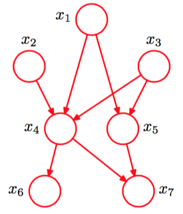
\includegraphics[scale=0.7]{pic/bayesian.png}
	\caption{较复杂的贝叶斯网络}
	\label{0-003}
\end{figure}
\end{frame}

\begin{frame}
	其联合概率分布可定义为:
	~\\
	~\\
	$P(x_1,...,x_7)=P(x_1)P(x_2)P(x_3)P(x_4|x_1,x_2,x_3)$
	\centerline{$\qquad\qquad p(x_5|x_2,x_3)P(x_6|x_4)P(x_7|x_4,x_5)$}
\end{frame}
	
\begin{frame}
	\begin{figure}
		\centering
		\begin{tabular}{ccc}
			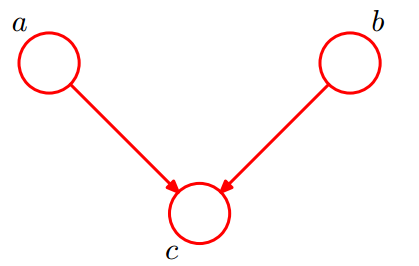
\includegraphics[width=0.28\linewidth]{pic/head2head.png} &
			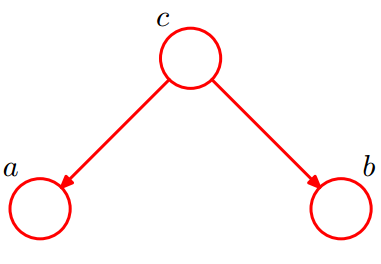
\includegraphics[width=0.28\linewidth]{pic/tail2tail.png} &
			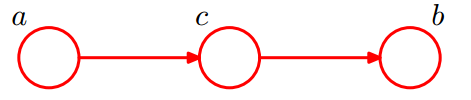
\includegraphics[width=0.28\linewidth]{pic/head2tail.png}\\
			(a) & (b) & (c) \\
			~\\
		\end{tabular}
		\caption{贝叶斯网络中属性的典型依赖关系}
		\label{0-004}
		\vspace{-0.5em}
	\end{figure}
\end{frame}

\begin{frame}
	(a)$\sum_{c}P(a,b,c)=\sum_{c}P(a)P(b)P(c|a,b)$ \\ $\Rightarrow P(a,b)=P(a)P(b)$
	~\\
	~\\
	(b)$P(a,b,c)=P(c)P(a|c)P(b|c)$ \\ $\Rightarrow P(a,b|c)=P(a|c)P(b|c)$
	~\\
	~\\
	(c)$P(a,b|c)=P(a,b,c)/P(c)$ \\ $\qquad\qquad\quad=P(a)P(c|a)P(b|c)/P(c)$ \\ $\qquad\qquad\quad=P(a,c)P(b|c)/P(c)$ \\ $\qquad\qquad\quad=P(a|c)P(b|c)$
\end{frame}

\subsection*{特点}
\begin{frame}
	\begin{itemize}
		\item贝叶斯网络的训练比较复杂,是一个 NP-complete问题,也就是说,现阶段没有可以在多项式时间内完成的算法。但是对于某些应用,这个训练过程可以简化,并在计算上高效实现。
		\item贝叶斯网络本身是一种不定性因果关联模型。它本身是将多元知识图解可视化的一种概率知识表达与推理模型,更为贴切地蕴含了网络节点变量之间的因果关系及条件相关关系。
		\item贝叶斯网络具有强大的不确定性问题处理能力。贝叶斯网络用条件概率表达各个信息要素之间的相关关系,能在有限的、不完整的、不确定的信息条件下进行学习和推理。
		\item贝叶斯网络能有效地进行多源信息表达与融合。贝叶斯网络可将故障诊断与维修决策相关的各种信息纳入网络结构中,按节点的方式统一进行处理,能有效地按信息的相关关系进行融合。
	\end{itemize}
\end{frame}

\subsection*{应用实例}
\begin{frame}
\begin{figure}
		\centering
		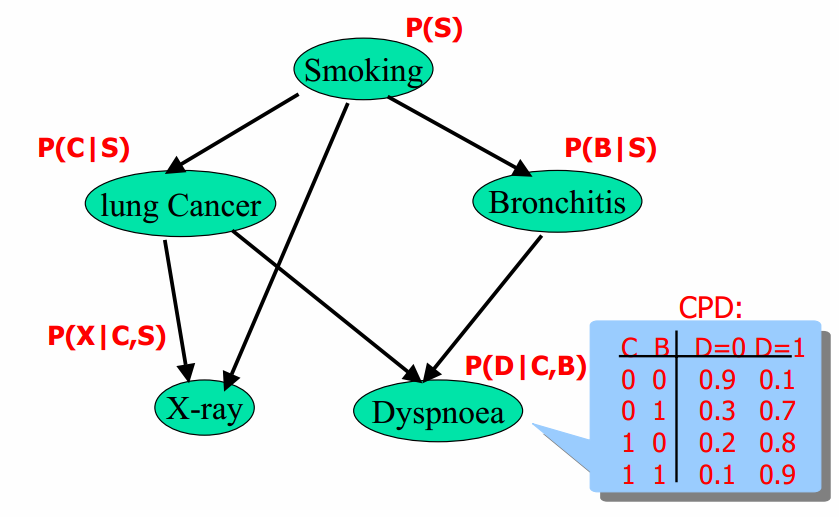
\includegraphics[scale=0.3]{pic/instance.png}
		\caption{贝叶斯网络实例}
		\label{0-005}
\end{figure}
\end{frame}

\subsection*{马尔科夫链}
\begin{frame}
	在给定$x_i$的条件下,$x_{i+1}$的分布与$x_1,x_2,...,x_{i-1}$无关,即$x_{i+1}$的分布只与$x_i$有关。这种顺次演变的随机过程,叫做马尔科夫链。马尔科夫链是贝叶斯网络的一种特例。
	~\\
	~\\
	\begin{figure}
		\centering
		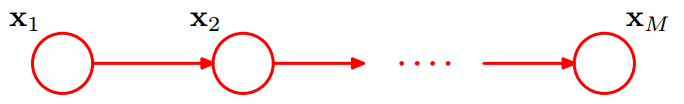
\includegraphics[scale=0.4]{pic/markov.png}
		\caption{马尔科夫链结构}
		\label{0-006}
	\end{figure}
\end{frame}

\begin{frame}
	马尔科夫链可表示为:
	~\\
	~\\
	\centerline{{\large $P(X_{n+1}=x|X_0,X_1,...,X_n)=P(X_{n+1}=x|X_n)$}}
	~\\
	~\\
	随机变量$X_1,X_2...$取值范围的合集成为“状态空间”,$X_i$的值表示在时间i的状态。马尔科夫链是时间和状态都是离散的马尔科夫过程。
\end{frame}

\begin{frame}
	如果状态空间是有限的,则转移概率分布可以表示为一个具有(i,j)元素的矩阵,称之为“转移矩阵”$\mathbf{P}$:
	~\\
	~\\
	\centerline{$P_{ij}=P(X_{n+1}=i|X_n=j)$}
	~\\
	对于一个离散状态空间,k步转移概率的积分即为求和,可以对转移矩阵求k次幂来求得。$\mathbf{P}^k$即是k步转移后的转移矩阵。\\平稳分布是一个满足以下方程的向量:
	~\\
	~\\
	\centerline{$\mathbf{P}\pi^*=\pi^*$}
	~\\
	在此情况下,稳态分布$\pi^*$是一个对应于特征根为1的、该转移矩阵的特征向量。
\end{frame}

	\section*{社交网络}

\begin{frame}
	\centerline{\textbf{\Large{社交网络}}} 
	~\\
	\centerline{\large{高一鸣}}
\end{frame}


\begin{frame}
	社交网络介绍
	
	\begin{itemize}
		\item 社交网络是由许多节点构成的一种社会结构
		\item 节点通常是指个人或组织
		\item 社交网络代表着各种社会关系
		\item 一个社交网络的大小最大约为150人左右,平均大小约为124人左右 
	\end{itemize}

\end{frame}

\begin{frame}
	发展
	\begin{itemize}
		\item 社交网络源自网络社交,网络社交的起点是电子邮件,解决了远程的邮件传输的问题
		\item BBS进一步把“群发”和“转发”常态化,实现了向所有人发布信息并讨论话题的功能
		\item 即时通信(IM)提高了即时效果(传输速度)和同时交流能力(并行处理)
		\item 博客(Blog)开始体现社会学和心理学的理论——信息发布节点开始体现越来越强的个体意识,因为在时间维度上的分散信息开始可以被聚合,进而成为信息发布节点的“形象”和“性格”
		\item 随着网络社交的演进,个人在网络上的形象更加趋于完整,社交网络就出现了
	\end{itemize}

\end{frame}

\begin{frame}
	阶段
	\begin{itemize}
		\item 早期概念化阶段──SixDegrees代表的六度分隔理论
		\item 结交陌生人阶段──Friendster帮你建立弱关系从而带来更高社会资本的理论
		\item 娱乐化阶段──MySpace创造的丰富的多媒体个性化空间吸引注意力的理论
		\item 社交图阶段──Facebook复制线下真实人际网络来到线上低成本管理的理论
		\item 云社交阶段——著云台分布式网际社交理论
	\end{itemize}

\end{frame}

\begin{frame}

	\begin{itemize}
		\item 整个SNS发展的过程是循着人们逐渐将线下生活的更完整的信息流转移到线上
		\item 网络社交一直在降低人们社交的时间和物质成本,降低管理和传递信息的成本
		\item 虚拟社交越来越与现实世界的社交出现交叉
		\item 网络社交已经开始承担大部分传统社交的作用
		\item 社交网络通过网络这载体,把人们连接起来,从而形成具有某一特点的团体
	\end{itemize}

\end{frame}

\begin{frame}
	社交网络理论
	\begin{itemize}
		\item 顿巴数(150定律)
		\item “六度分隔”理论
		\item 贝肯数
		\item 强弱关系链
		\item 二八定律
		\item 马太效应
		\item 长尾效应
		\item 羊群效应
		\item 马斯洛需求模型
	\end{itemize}

\end{frame}

\begin{frame}
	\textbf{顿巴数(150定律)}
	
	人类大脑的逻辑和记忆力结构,注定了大脑可以容纳148人的稳定社交关系,四舍五入大约是150人。
	
	当社会群组超过150人的就无法有效地沟通和协作。
	
	人类的社会结构表现为:
	\begin{itemize}
		\item 5人左右的亲密接触圈
		\item 12-15人的同情圈,即如果这一圈里有人去世,会感到伤心
		\item 50人左右的群落,即经常一起生活、一起行动的人
		\item 150人左右的氏族,即遵从共同仪式的人
		\item 500人左右的部落,即拥有同种语言的人
		\item 5000人左右的群落,即有共同文化的人
	\end{itemize}

\end{frame}

\begin{frame}

	\begin{figure}[htbp]
		\centering
		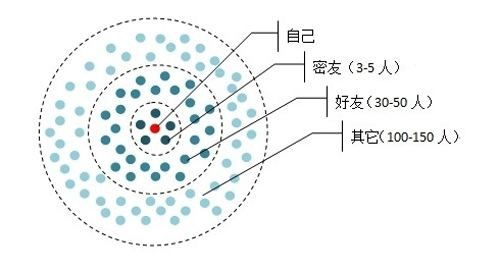
\includegraphics[width=0.8\textwidth]{pic/t1.jpg}
		\caption{顿巴数同心圆模型}
	\end{figure}
	当社会结构的人数超过150人时,相互间的互动和影响就会减少很多,只能靠共同的语言来维系。
	
	当人数上升到5000人左右时,只能依靠共同的文化维系社会结构。

\end{frame}

\begin{frame}
	\textbf{“六度分隔”理论}
	
	"六度分隔"现象,又称为“小世界现象”。
	
	可通俗地阐述为:你和任何一个陌生人之间所间隔的人不会超过五个,最多通过五个人你就能够认识任何一个陌生人。
	\begin{itemize}
		\item 数学解释:若每个人平均认识260人,其六度就是260的(6-1)次幂为1,188,137,600,000,几乎覆盖了整个地球人口
		\item 奠定了社交网络的理论基础
		\item 社会化的现代人类社会成员之间,都可能通过“六度空间”而联系起来,绝对没有联系的A与B是不存在的
	\end{itemize}

\end{frame}

\begin{frame}

	\begin{figure}[htbp]
		\centering
		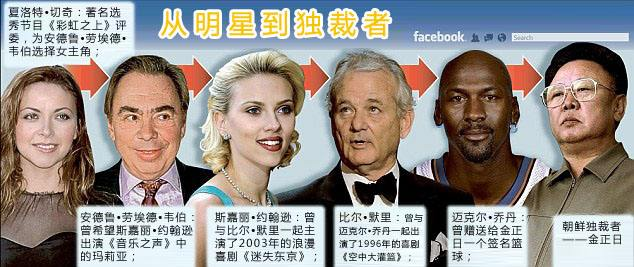
\includegraphics[width=0.8\textwidth]{pic/t2.jpg}
		\caption{"六度分隔"现象}
	\end{figure}

\end{frame}

\begin{frame}
	\textbf{贝肯数}
	
	凯文贝肯与好莱坞的影视明星发生联系所需要的中间人数量即为“贝肯数”。
	
	弗吉尼亚大学一个实验室曾为约25万上过银幕的男女演员计算了“平均贝肯数”,所有人的贝肯数都在2.6和3之间,并且相差十分微小。
	\begin{itemize}
		\item 证明想进入网络的链接中心,并不一定要成为大人物,成为一个“永不退场”的配角也可以非常接近网络的中心,因为和中心人物的距离其实可以近到忽略不计
		\item 证明一个网络社区的崩溃,不会因为多少普通用户流失而发生,但几个高链接节点用户的流失,就会造成崩溃
		\item 虽然六度分隔理论将大多数人相连,但是总有那些掌握着重要人脉的节点,通过那些节点六度空间才能顺利形成通路
	\end{itemize}

\end{frame}

\begin{frame}

	\begin{figure}[htbp]
		\centering
		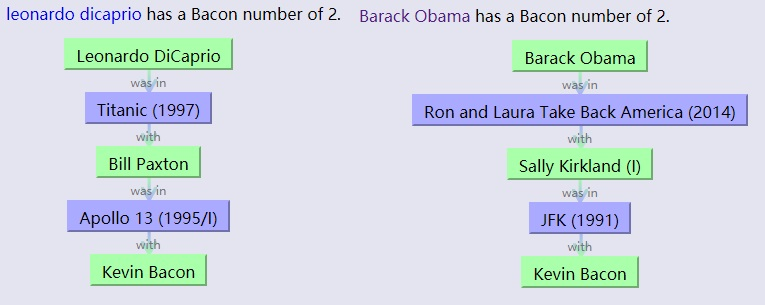
\includegraphics[width=0.9\textwidth]{pic/t3.jpg}
		\caption{贝肯数例子}
	\end{figure}

\end{frame}

\begin{frame}
	\textbf{强弱关系链}
	
	在传统社会,每个人接触最频繁的是自己的亲人、同学、朋友、同事等,这是一种十分稳定的然而范围有限的社会关系,称为“强关系” ;同时,还存在另外一类相对于前一种社会关系较浅,然而却是更为广泛的社会关系,称为"弱关系"。
	
	强连接关系通常表明行动者彼此之间具有高度的互动,在某些存在的互动关系型态上较亲密。因此,透过强关系所产生的讯息通常是重复的,容易自成一个封闭的系统,故认为在组织中强关系网络并不是一个可以提供创新机会的渠道。
	
	弱关系在我们与外界交流时发挥了关键的作用,为了得到新的信息,我们必须充分发挥弱关系的作用。弱关系是与外界沟通的桥梁,不同地方的人通过弱关系可以得到不同的信息。
	
	强弱关系并不仅由人与人之间的关系类型决定,还会由六度理论的度数决定,例如1度关系比2度关系强。

\end{frame}

\begin{frame}

	\begin{figure}[htbp]
		\centering
		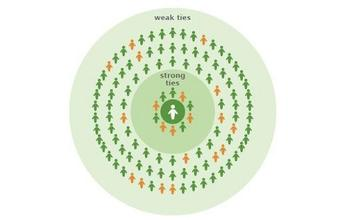
\includegraphics[width=0.9\textwidth]{pic/t4.jpg}
		\caption{强弱关系链}
	\end{figure}

\end{frame}


\begin{frame}
	\textbf{二八定律}
	
	在任何一组东西中,最重要的只占其中一小部分,约20\%,其余80\%的尽管是多数,却是次要的,因此又称二八定律。
	
	二八定律可以延伸到各个领域,包括人脉,例如20\%的人脉给你带来80\%的价值

\end{frame}

\begin{frame}

	\begin{figure}[htbp]
		\centering
		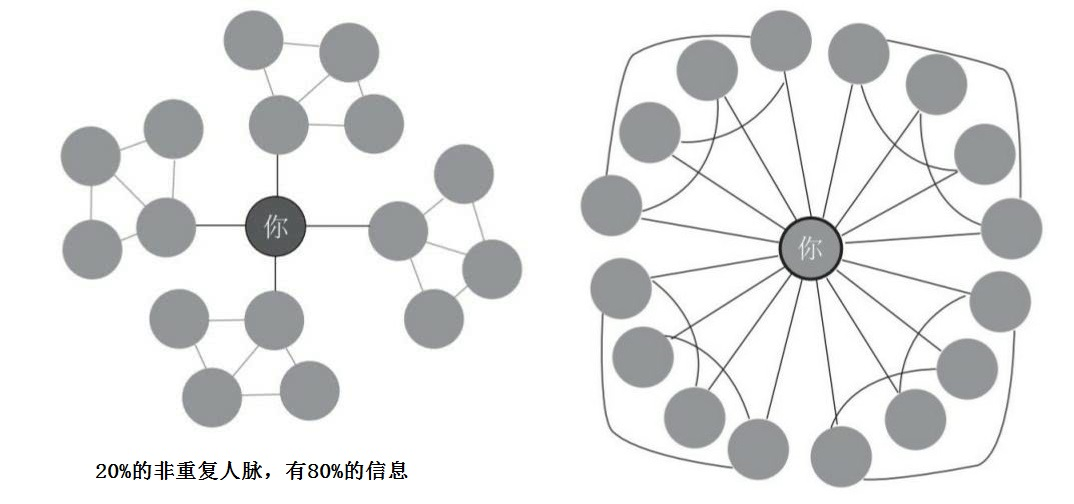
\includegraphics[width=0.9\textwidth]{pic/t5.jpg}
		\caption{二八定律}
	\end{figure}

\end{frame}

\begin{frame}
	\textbf{马太效应}
	
	任何个体、群体或地区,在某一个方面(如金钱、名誉、地位等)获得成功和进步,就会产生一种积累优势,就会有更多的机会取得更大的成功和进步。
	
	马太效应揭示了一个大概率事件:社交网络中重要的节点很可能会越来越重要,而位于网络边缘的节点,可能会越来越被弱化。
	
	社会交往中,那些长于交际朋友多的人会借助频繁的交往,认识更多的朋友;那些内向沉默的人则会越来越孤独。
	
\end{frame}

\begin{frame}

	\begin{figure}[htbp]
		\centering
		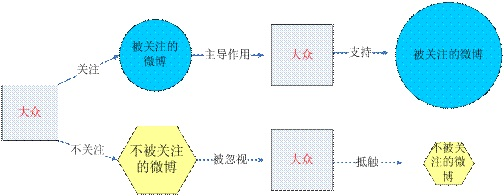
\includegraphics[width=0.9\textwidth]{pic/t6.jpg}
		\caption{马太效应例子}
	\end{figure}

\end{frame}

\begin{frame}
	\textbf{长尾效应}
	
	“头”(head)和“尾”(tail)是两个统计学名词。正态曲线中间的突起部分叫“头”;两边相对平缓的部分叫“尾”。
	
	对于社交网络来说,并不是八成不重要的节点就没有用。虽然社交网络中存在不太重要的节点,但是对于一个覆盖面很广的社交网络来说,八成重要性并不是最重要的节点也有其商业开发的价值,互联网的浪潮已经将商品成本降至极低,长尾理论将发挥巨大的价值。
	
\end{frame}

\begin{frame}

	\begin{figure}[htbp]
		\centering
		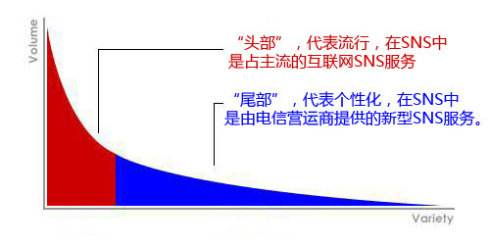
\includegraphics[width=0.9\textwidth]{pic/t7.jpg}
		\caption{长尾效应}
	\end{figure}

\end{frame}

\begin{frame}
	\textbf{羊群效应}
	
	“羊群效应”也叫“从众效应”:是个人的观念或行为由于真实的或想象的群体的影响或压力,而向与多数人相一致的方向变化的现象。
	
	无论构成这个群体的个人是谁,他们的生活方式、职业、性格、智力有多么的相似或者不相似,只要他们构成了一个群体,他们的感觉、思考、行为方式就会和他们处于独立状态时有很大的不同。
	
	社交网络中的节点都会互相影响,每个个体都会偏向大多数人的判断,每个个体都有从众的趋向性。
\end{frame}

\begin{frame}
	\textbf{马斯洛需求模型}
	
	将人类需求像阶梯一样从低到高按层次分为五种,分别是:生理需求、安全需求、社交需求、尊重需求和自我实现需求。
	
	需求层次理论有两个基本出发点,一是人人都有需要,某层需要获得满足后,另一层需要才出现;二是在多种需要未获满足前,首先满足迫切需要,该需要满足后,后面的需要才显示出其激励作用。
	
	社交网络中的节点是千差万别的,节点间的联系是多种多样的,但归根结底,社交网络是因为满足每个个体的需求而存在,并基于需求模型而发展演变。
\end{frame}

\begin{frame}

	\begin{figure}[htbp]
		\centering
		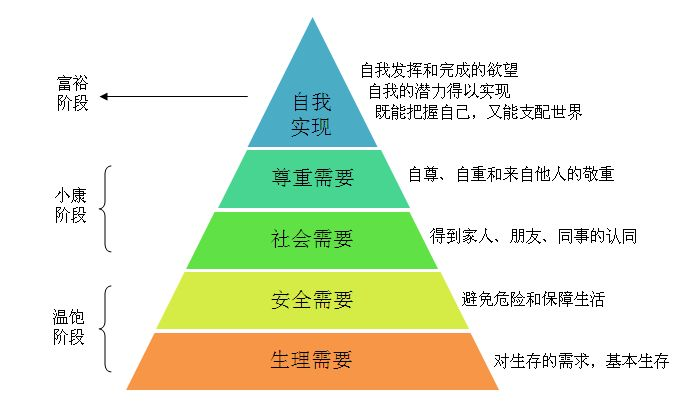
\includegraphics[width=0.9\textwidth]{pic/t9.jpg}
		\caption{马斯洛需求模型}
	\end{figure}

\end{frame}

\begin{frame}
	\textbf{基本要素}
	
	社交网络模型许多概念来自于图论,因为社交网络模型本质上是一个由节点(人)和边(社交关系)组成的图。主要包括以下要素:
	\begin{itemize}
		\item 节点(Node):节点是指要分析的物体,每一个物体就是一个节点,比如在Social Network中每个人就是一个节点。
		\item 边(Edge):Graph中两个节点间的连线,用于表示两个节点的关系。比如在Social Network中两个人的关注关系,微博传播中转发关系。
		\item 图是用来表示一组物体之间的关系的方式。有向图(Directed Graph):边代表的关系具有方向的图。比如微博的关注关系,电话拨入呼出,银行转账收账就是有方向的。无向图(Undirected Graph):边代表的关系没有方向的图。
		\item 度(Degree):节点的度是指与其相连的边数,你通讯录的名单长度就是你的联络人度数。网络平均度反应了网络的疏密程度,而通过度分布则可以刻画不同节点的重要性。
	\end{itemize}

\end{frame}

\begin{frame}
	\textbf{基本要素}
	
	\begin{itemize}
		\item 输入度(In-degree):有向图中一个节点收到的边。
		\item 输出度(Out-degree):有向图中一个节点发出的边。
		\item 路径(Route): 两个节点之间经过的边和节点序列,路径有长度,通常衡量两个点之间的距离。
		\item 网络密度(Density):网络密度可以用于刻画节点间相互连边的密集程度,定义为网络中实际存在边数与可容纳边数上限的比值,常用来测量社交网络中社交关系的密集程度及演化趋势。
		\item 聚类系数(Clustering Coefficient):用于描述网络中与同一节点相连的节点间也互为相邻节点的程度。其用于刻画社交网络中一个人朋友们之间也互相是朋友的概率,反应了社交网络中的聚集性。
		\item 介数(Betweeness):为图中某节点承载整个图所有最短路径的数量,通常用来评价节点的重要程度,比如在连接不同社群之间的中介节点的介数相对于其他节点来说会非常大,也体现了其在社交网络信息传递中的重要程度。
	\end{itemize}

\end{frame}

\begin{frame}
	\textbf{网络特性}
	
	\begin{itemize}
		\item 小世界现象:小世界现象是指地理位置相距遥远的人可能具有较短的社会关系间隔。小世界现象在在线社交网络中得到了很好地验证,根据2011年 Facebook 数据分析小组的报告, Facebook 约7.2亿用户中任意两个用户间的平均路径长度仅为4.74,而这一指标在推特中为4.67。可以说,在五步之内,任何两个网络上的个体都可以互相连接。
		
		\item 无标度特性:大多数真实的大规模社交网络都存在着大多数节点有少量边,少数节点有大量边的特点,其网络缺乏一个统一的衡量尺度而呈现出异质性,我们将这种节点度分布不存在有限衡量分布范围的性质称为无标度。无标度网络表现出来的度分布特征为幂律分布,这就是此类网络的无标度特性。
	\end{itemize}

\end{frame}

\begin{frame}
	\textbf{网络模型}
	
	规则图:有n个节点,每个节点有d个邻居节点,每个节点只和邻居节点相连。
	
	ER随机图:有n个节点,每个节点以概率p连接n个节点。
\end{frame}

\begin{frame}
	WS模型:有n个节点,每个节点有k个邻居,每个节点先和周围的邻居节点相连,然后以概率p随机地重新连接网络中的每个边,即将边的一个端点保持不变,而另一个端点取为网络中随机选择的一个节点(其中规定,任意两个不同的节点之间至多只能有一条边,并且每一个节点都不能有边与自身相连)。
	\begin{figure}[htbp]
		\centering
		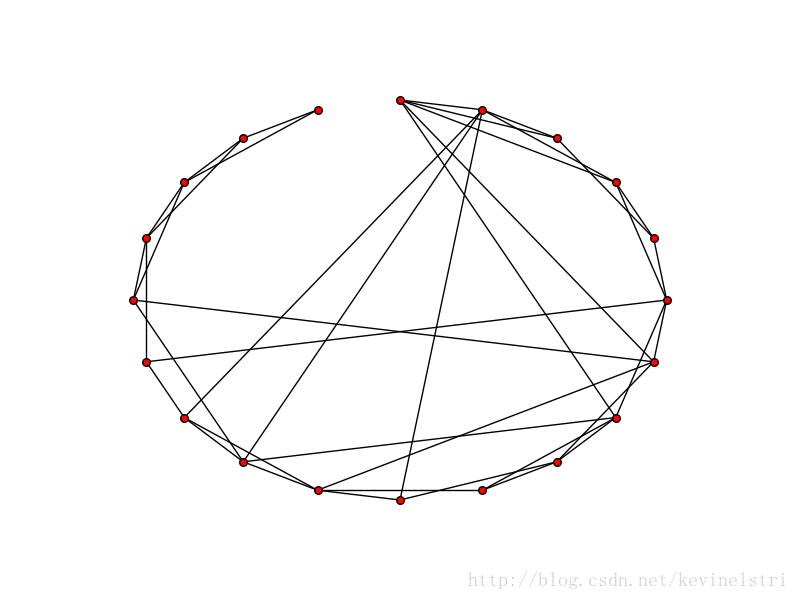
\includegraphics[width=0.6\textwidth]{pic/WS.png}
		\caption{WS模型}
	\end{figure}
\end{frame}

\begin{frame}
	BA模型:开始有0个节点,每次加入一个节点,并以一定概率(概率和已有节点的度是成正比的,度越大的节点越有可能被连接)与已存在的m个节点相连,直到有n个点。BA模型考虑到现实网络中节点的幂律分布特性,生成无标度网络。
	\begin{figure}[htbp]
		\centering
		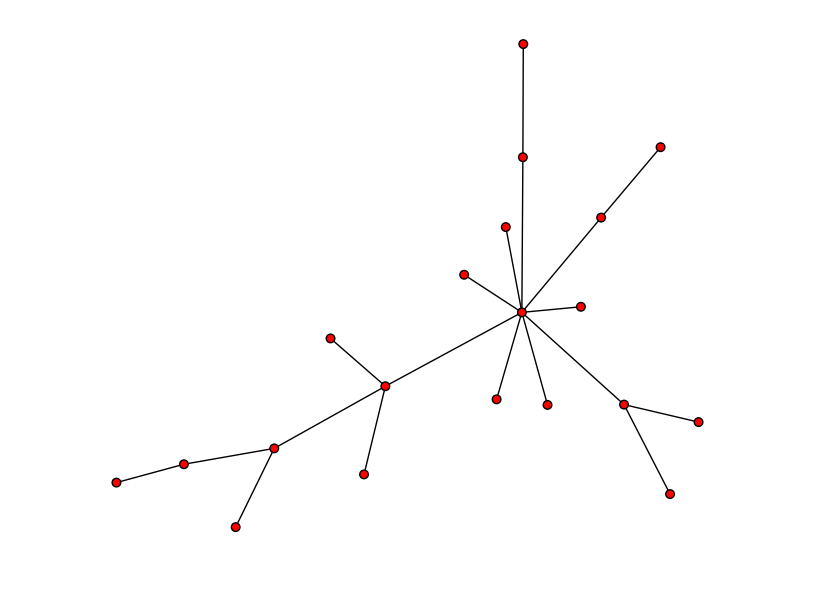
\includegraphics[width=0.6\textwidth]{pic/BA.png}
		\caption{BA模型}
	\end{figure}
\end{frame}
\begin{frame}
	\textbf{社区发现算法}
	
	社区发现:在图中发现n个社区,同一个社区内的连接紧密,而社区间的连接非常稀疏。
\end{frame}

\begin{frame}
	\textbf{GN算法}
	
	边介数(betweenness):网络中经过该边的最短路径占所有最短路径的比例。
	\begin{itemize}
		\item 计算网络中所有边的介数
		\item 找到介数最高的边,并将它从网络中移除 
		\item 重复以上步骤,直到每个节点就是一个社区为止
	\end{itemize}
	
	\begin{figure}[htbp]
		\centering
		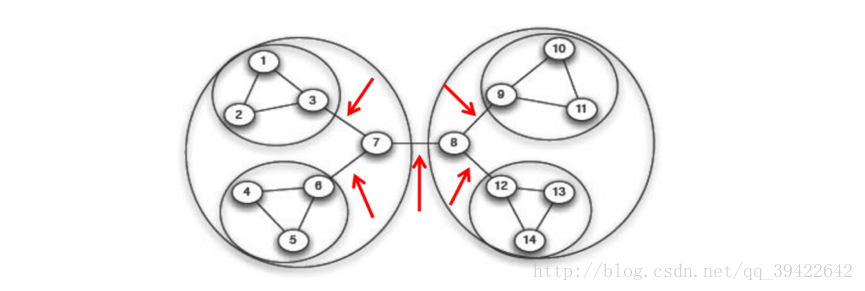
\includegraphics[width=0.8\textwidth]{pic/GN.png}
	\end{figure}
\end{frame}

\begin{frame}
	\textbf{Louvain算法}
	
	Louvain算法是基于模块度的算法,其优化目标就是最大化整个社区网络结构的模块度。
	
	模块度:物理含义是社区内节点的连边数与随机情况下节点的连边数之差,它可以衡量一个社区紧密程度的度量。
	
	\begin{figure}[htbp]
		\centering
		
\includegraphics[width=0.8\textwidth]{pic/Louvain.png}
	\end{figure}

	\begin{itemize}
		\item 不断遍历网络中的节点,尝试把单个节点加入能使模块度提升最大的社区,直到所有节点不再改变 
		\item 将第一阶段形成的一个个小的社区并为一个节点,重新构造网络。(边的权重为两个节点内所有原始节点的边权重之和)
		\item 重复以上两步
	\end{itemize}
\end{frame}

\begin{frame}
	\textbf{LPA算法}
	
	\begin{itemize}
		\item 初始化每个节点,并赋予唯一标签 
		\item 根据邻居节点最常见的标签更新每个节点的标签 
		\item 最终收敛后标签一致的节点属于同一社区
	\end{itemize}
\end{frame}

	\section*{马尔科夫场}

\begin{frame}
	\centerline{\textbf{\Large{马尔科夫场}}} 
	~\\
	\centerline{\large{王方正}}
\end{frame}

\subsection*{模型定义}
\begin{frame}
	马尔科夫随机场,又称为概率无向图模型,是一个可以由无向图表示的联合概率分布。
\end{frame}

\begin{frame}

	\begin{block}{图}
		图是由结点及连接结点的边组成的集合。结点和边分别记作$v$和$e$,结点和边的集合分别记作$V$和$E$,图记作$G=(V,E)$。\\
		无向图是指边没有方向的图。
	\end{block}

	\begin{block}{概率图模型}
		概率图模型(PGM)是由图表示的概率分布。设有联合概率分布$P(Y)$,$Y\in\mathcal{Y}$是一组随机变量。由无向图$G=(V,E)$表示概率分布,即在图$G$中,结点$v\in V$表示一个随机变量$Y_v$,$Y=(Y_v)_{v\in V}$;边$e\in E$表示随机变量之间的概率依赖关系。
	\end{block}

\end{frame}

\begin{frame}
	马尔可夫性:三者等价
	
	\begin{itemize}
		\item 成对马尔可夫性:$P(Y_u,Y_v|Y_O)=P(Y_u|Y_O)P(Y_v|Y_O)$
		\item 局部马尔可夫性:$P(Y_v,Y_O|Y_W)=P(Y_v|Y_W)P(Y_O|Y_W)$
		\item 全局马尔可夫性:$P(Y_A,Y_B|Y_C)=P(Y_A|Y_C)P(Y_B|Y_C)$
	\end{itemize}

\end{frame}

\begin{frame}

	\begin{figure}[htbp]
		\centering
		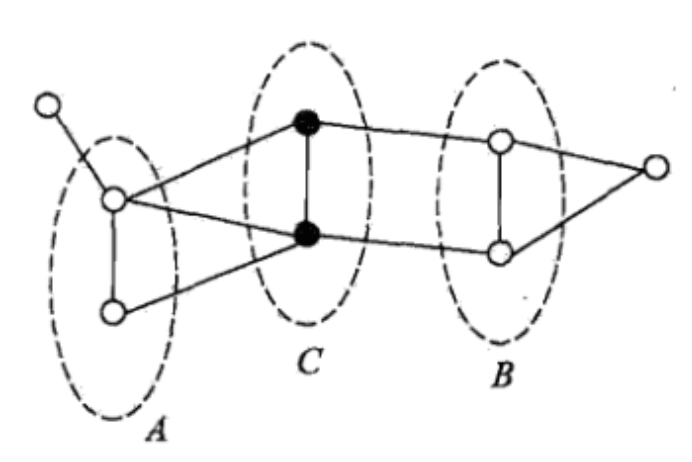
\includegraphics[scale=0.6]{pic/1-1.png}
		\caption{局部马尔可夫性}
		\label{1-001}
	\end{figure}

\end{frame}

\begin{frame}

	\begin{figure}[htbp]
		\centering
		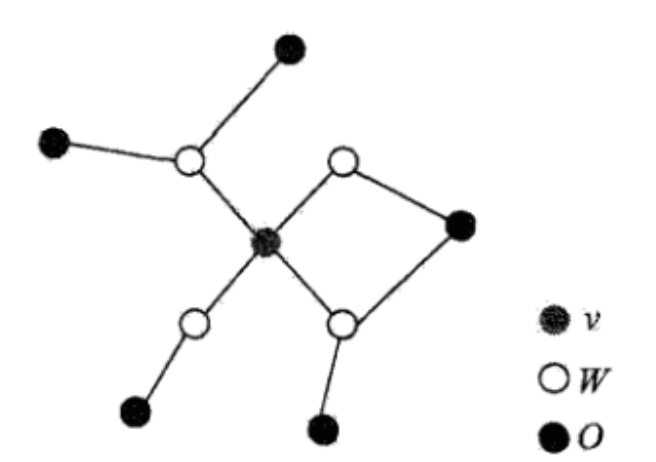
\includegraphics[scale=0.6]{pic/1-2.png}
		\caption{全局马尔可夫性}
		\label{1-002}
	\end{figure}

\end{frame}

\begin{frame}

	\begin{block}{概率无向图模型}
		设有联合概率分布$P(Y)$ ,由无向图$G=(V,E)$表示,在图$G$中,结点表示随机变量,边表示随机变量之间的依赖关系。如果联合概率分布$P(Y)$满足成对、局部或全局马尔可夫性,就称此联合概率分布为概率无向图模型或马尔可夫随机场。
	\end{block}

\end{frame}

\subsection*{因子分解}

\begin{frame}

	\begin{block}{团}
		无向图$G$中任何两个结点均有边连接的结点子集称为团。
	\end{block}
	
	\begin{block}{最大团}
		若$C$是无向图$G$的一个团,并且不能再加进任何一个$G$的结点使其成为一个更大的团,则称此$C$为最大团。
	\end{block}

\end{frame}

\begin{frame}

	\begin{figure}[htbp]
		\centering
		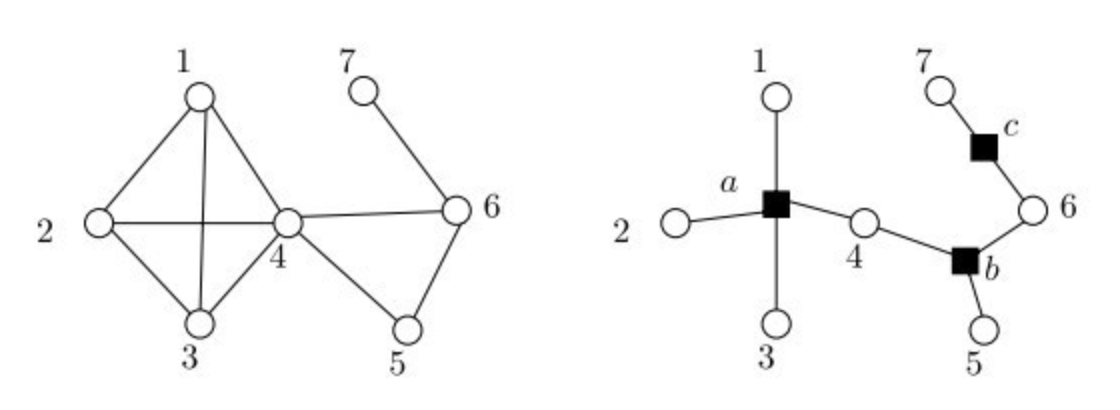
\includegraphics[scale=0.6]{pic/1-3.png}
		\caption{无向图与因子图}
		\label{1-003}
	\end{figure}

\end{frame}

\begin{frame}

	将概率无向图模型的联合概率分布表示为其最大团上的随机变量的函数的乘积形式的操作,称为概率无向图模型的因子分解。具体公式为:
	$$P(Y)=\frac{1}{Z}\prod_{C}\Psi_{C}(Y_C)$$
	其中,Z是规范化因子,由式
	$$Z=\sum_{Y}\prod_{C}\Psi_{C}(Y_C)$$
	给出。规范化因子保证$P(Y)$构成一个概率分布。\\
	函数$\Psi_{C}(Y_C)$称为势函数,通常定义为指数函数:
	$$\Psi_{C}(Y_C)=exp^{-E(Y_C)}$$
	势函数的作用是刻画变量之间的相关关系,它是非负函数,并且在所偏好的变量取值上有较大函数值。

\end{frame}

\subsection*{应用}

\begin{frame}

	\begin{figure}[htbp]
		\centering
		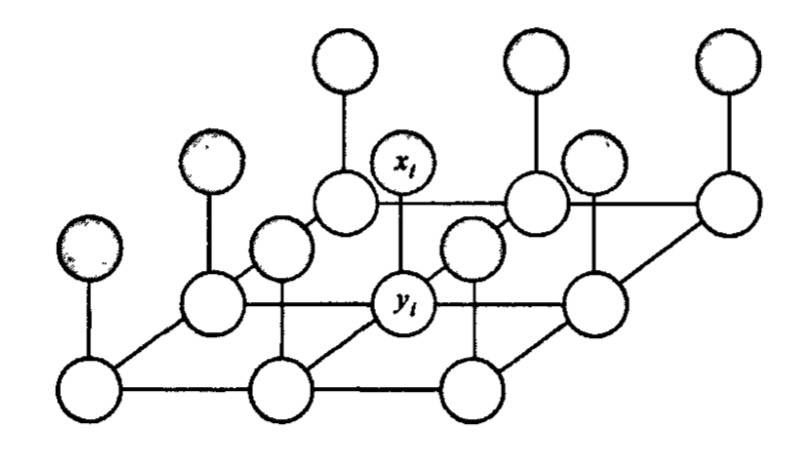
\includegraphics[scale=0.6]{pic/1-4.png}
		\caption{Pairwise MRF 模型}
		\label{1-004}
	\end{figure}

\end{frame}











\end{document}
